%!TEX root = ../main.tex
\chapter{Bonnes Pratiques --- Tests, Documentation, Git}
\label{ch:bonnes_pratiques}

\begin{intuition}
\'Ecrire du code qui fonctionne est une chose ; \'ecrire du code \textbf{fiable},
\textbf{lisible} et \textbf{reproductible} en est une autre. En science, un r\'esultat
doit \^etre v\'erifiable et reproductible. Ce chapitre pr\'esente les outils et
m\'ethodes qui font la diff\'erence entre un script jetable et un projet scientifique
de qualit\'e : style de code, documentation, tests et contr\^ole de version.
\end{intuition}

% ----------------------------------------------------------------
\section{Style de code : PEP\,8}
\index{PEP 8}\index{style de code}

\begin{definition}[PEP\,8]
\textbf{PEP\,8} est le guide de style officiel de Python. Il d\'efinit des conventions
de nommage, d'indentation et de mise en forme pour rendre le code lisible et
coh\'erent.
\end{definition}

\begin{codeblock}[title=\textbf{Python}]
\begin{minted}{python}
# MAUVAIS STYLE
def f(x,y,z):
    A=x*y+z
    if(A>10):
        return A
    else:
        return A*2

# BON STYLE (PEP 8)
def calculer_score(longueur, largeur, bonus):
    """Calcule le score en fonction des dimensions et du bonus."""
    score = longueur * largeur + bonus
    if score > 10:
        return score
    else:
        return score * 2
\end{minted}
\end{codeblock}

\begin{bonnepratique}
R\`egles essentielles de PEP\,8 :
\begin{itemize}
  \item \textbf{Indentation} : 4 espaces (jamais de tabulations).
  \item \textbf{Longueur de ligne} : maximum 79 caract\`eres.
  \item \textbf{Noms de variables} : \py{snake\_case} (ex. : \py{masse\_molaire}).
  \item \textbf{Noms de classes} : \py{CamelCase} (ex. : \py{ParticuleChargee}).
  \item \textbf{Constantes} : \py{MAJUSCULES} (ex. : \py{VITESSE\_LUMIERE}).
  \item \textbf{Espaces autour des op\'erateurs} : \py{x = 3 + y}, pas \py{x=3+y}.
\end{itemize}
\end{bonnepratique}

\begin{codeblock}[title=\textbf{Python}]
\begin{minted}{python}
# Conventions de nommage
CONSTANTE_BOLTZMANN = 1.380649e-23   # Constante (MAJUSCULES)
temperature_kelvin = 300.0            # Variable (snake_case)

class MoleculeGaz:                    # Classe (CamelCase)
    def __init__(self, masse, vitesse):
        self.masse = masse
        self.vitesse = vitesse

    def energie_cinetique(self):      # M\'ethode (snake_case)
        return 0.5 * self.masse * self.vitesse**2
\end{minted}
\end{codeblock}

% ----------------------------------------------------------------
\section{Docstrings et documentation}
\index{docstring}\index{documentation}

Une \textbf{docstring} est une cha\^ine de documentation plac\'ee juste apr\`es la
d\'efinition d'une fonction, d'une classe ou d'un module.

\begin{codeblock}[title=\textbf{Python}]
\begin{minted}{python}
def energie_cinetique(masse, vitesse):
    """
    Calcule l'\'energie cin\'etique d'un objet.

    Parameters
    ----------
    masse : float
        Masse de l'objet en kilogrammes (kg).
    vitesse : float
        Vitesse de l'objet en m\`etres par seconde (m/s).

    Returns
    -------
    float
        \'Energie cin\'etique en joules (J).

    Examples
    --------
    >>> energie_cinetique(2.0, 3.0)
    9.0
    """
    return 0.5 * masse * vitesse**2
\end{minted}
\end{codeblock}

\begin{codeblock}[title=\textbf{Python}]
\begin{minted}{python}
# Acc\'eder `a la documentation
help(energie_cinetique)
\end{minted}
\end{codeblock}

\begin{codeoutput}
\begin{verbatim}
Help on function energie_cinetique in module __main__:

energie_cinetique(masse, vitesse)
    Calcule l'energie cinetique d'un objet.

    Parameters
    ----------
    masse : float
        Masse de l'objet en kilogrammes (kg).
    vitesse : float
        Vitesse de l'objet en metres par seconde (m/s).

    Returns
    -------
    float
        Energie cinetique en joules (J).
\end{verbatim}
\end{codeoutput}

\begin{remarque}
Le style utilis\'e ci-dessus s'appelle le \textbf{style NumPy}\index{style NumPy}.
C'est le standard dans l'\'ecosyst\`eme scientifique Python. D'autres styles existent
(Google, Sphinx), mais le style NumPy est le plus r\'epandu en sciences.
\end{remarque}

% ----------------------------------------------------------------
\section{Tests avec \py{assert}}
\index{assert}\index{tests}

Tester son code, c'est comme v\'erifier une mesure exp\'erimentale : on compare
le r\'esultat obtenu au r\'esultat attendu.

\begin{codeblock}[title=\textbf{Python}]
\begin{minted}{python}
def celsius_vers_kelvin(temp_c):
    """Convertit une temp\'erature de Celsius en Kelvin."""
    return temp_c + 273.15

# Tests simples avec assert
assert celsius_vers_kelvin(0) == 273.15, "Erreur : 0°C != 273.15 K"
assert celsius_vers_kelvin(100) == 373.15, "Erreur : 100°C"
assert celsius_vers_kelvin(-273.15) == 0.0, "Erreur : z\'ero absolu"
print("Tous les tests sont pass\'es !")
\end{minted}
\end{codeblock}

\begin{codeoutput}
\begin{verbatim}
Tous les tests sont passes !
\end{verbatim}
\end{codeoutput}

\begin{codeblock}[title=\textbf{Python}]
\begin{minted}{python}
import math

def aire_cercle(rayon):
    """Calcule l'aire d'un cercle."""
    if rayon < 0:
        raise ValueError("Le rayon doit \^etre positif.")
    return math.pi * rayon**2

# Tests
assert abs(aire_cercle(1) - math.pi) < 1e-10
assert abs(aire_cercle(0) - 0) < 1e-10
assert abs(aire_cercle(2) - 4 * math.pi) < 1e-10

# Test de l'exception
try:
    aire_cercle(-1)
    assert False, "Aurait d\^u lever une erreur"
except ValueError:
    pass  # C'est le comportement attendu

print("Tous les tests sont pass\'es !")
\end{minted}
\end{codeblock}

\begin{codeoutput}
\begin{verbatim}
Tous les tests sont passes !
\end{verbatim}
\end{codeoutput}

\begin{attention}
Pour les nombres \`a virgule flottante, ne testez \emph{jamais} l'\'egalit\'e exacte.
Utilisez une tol\'erance : \py{abs(obtenu - attendu) < 1e-10} ou
\py{math.isclose(obtenu, attendu)}.
\end{attention}

% ----------------------------------------------------------------
\section{Contr\^ole de version avec Git}
\index{Git}\index{contr\^ole de version}

\begin{definition}[Git]
\textbf{Git} est un syst\`eme de contr\^ole de version distribu\'e. Il enregistre
l'historique complet des modifications d'un projet, permettant de revenir en
arri\`ere, de collaborer et de travailler sur des branches parall\`eles.
\end{definition}

\begin{center}
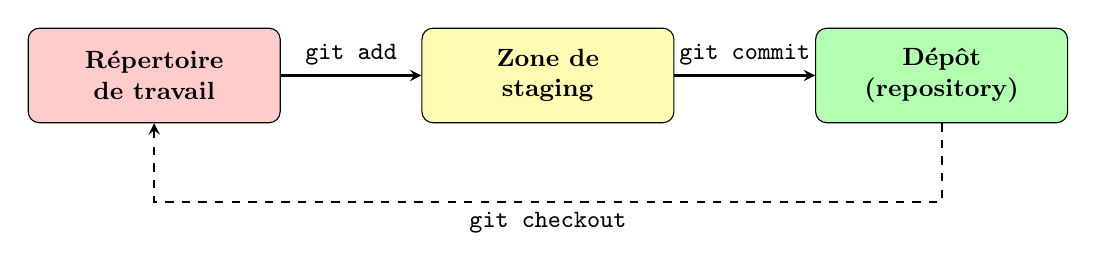
\begin{tikzpicture}[
  block/.style={draw, rounded corners, minimum width=3.2cm, minimum height=1.2cm,
                align=center, font=\small},
  arr/.style={->, thick, >=stealth},
]
  \node[block, fill=red!20] (wd) at (0,0) {\textbf{R\'epertoire}\\\textbf{de travail}};
  \node[block, fill=yellow!30] (stage) at (5,0) {\textbf{Zone de}\\\textbf{staging}};
  \node[block, fill=green!30] (repo) at (10,0) {\textbf{D\'ep\^ot}\\\textbf{(repository)}};

  \draw[arr] (wd.east) -- (stage.west) node[midway, above, font=\ttfamily\small] {git add};
  \draw[arr] (stage.east) -- (repo.west) node[midway, above, font=\ttfamily\small] {git commit};
  \draw[arr, dashed] (repo.south) -- ++(0,-1) -| (wd.south)
    node[pos=0.25, below, font=\ttfamily\small] {git checkout};
\end{tikzpicture}
\end{center}

\begin{codeblock}[title=\textbf{Python}]
\begin{minted}{python}
# Commandes Git essentielles (dans le terminal)
# Ces commandes sont ex\'ecut\'ees dans un shell, pas en Python

# 1. Initialiser un d\'ep\^ot
# $ git init

# 2. V\'erifier l'\'etat
# $ git status

# 3. Ajouter des fichiers
# $ git add analyse.py
# $ git add .              # Tout ajouter

# 4. Enregistrer (commit)
# $ git commit -m "Ajout de l'analyse initiale"

# 5. Consulter l'historique
# $ git log --oneline
\end{minted}
\end{codeblock}

\begin{exemple}[Session Git typique]
\begin{codeblock}[title=\textbf{Python}]
\begin{minted}{python}
# Voici une session Git typique dans le terminal :
#
# $ mkdir mon_projet && cd mon_projet
# $ git init
# Initialized empty Git repository in .../mon_projet/.git/
#
# $ echo "print('Bonjour')" > main.py
# $ git add main.py
# $ git commit -m "Premier commit : script principal"
# [master (root-commit) a1b2c3d] Premier commit : script principal
#
# $ echo "# Mon Projet" > README.md
# $ git add README.md
# $ git commit -m "Ajout du README"
#
# $ git log --oneline
# b4e5f6g Ajout du README
# a1b2c3d Premier commit : script principal
\end{minted}
\end{codeblock}
\end{exemple}

% ----------------------------------------------------------------
\section{Environnements virtuels}
\index{venv}\index{environnement virtuel}

\begin{definition}[Environnement virtuel]
Un \textbf{environnement virtuel} est un r\'epertoire isol\'e contenant une installation
Python ind\'ependante. Chaque projet peut ainsi avoir ses propres d\'ependances sans
conflit avec d'autres projets.
\end{definition}

\begin{codeblock}[title=\textbf{Python}]
\begin{minted}{python}
# Cr\'eer un environnement virtuel
# $ python -m venv mon_env

# L'activer
# Linux/Mac :   $ source mon_env/bin/activate
# Windows :     $ mon_env\Scripts\activate

# Installer des paquets
# (mon_env) $ pip install numpy scipy matplotlib

# Sauvegarder les d\'ependances
# (mon_env) $ pip freeze > requirements.txt

# Reproduire l'environnement ailleurs
# $ pip install -r requirements.txt
\end{minted}
\end{codeblock}

\begin{bonnepratique}
Cr\'eez \textbf{toujours} un environnement virtuel pour chaque projet.
Ajoutez le dossier de l'environnement (\texttt{mon\_env/}) au fichier
\texttt{.gitignore} pour ne pas le versionner.
\end{bonnepratique}

% ----------------------------------------------------------------
\section{Structure d'un projet scientifique}
\index{structure de projet}

\begin{codeblock}[title=\textbf{Python}]
\begin{minted}{python}
# Structure recommand\'ee pour un projet scientifique
#
# mon_projet/
# |-- README.md              # Description du projet
# |-- requirements.txt       # D\'ependances
# |-- .gitignore             # Fichiers `a ignorer
# |-- src/
# |   |-- __init__.py
# |   |-- analyse.py         # Fonctions d'analyse
# |   |-- visualisation.py   # Fonctions de trac\'e
# |-- tests/
# |   |-- test_analyse.py    # Tests unitaires
# |-- data/
# |   |-- mesures.csv        # Donn\'ees brutes
# |-- notebooks/
# |   |-- exploration.ipynb  # Carnets Jupyter
# |-- resultats/
#     |-- figures/            # Graphiques g\'en\'er\'es
\end{minted}
\end{codeblock}

\begin{codeblock}[title=\textbf{Python}]
\begin{minted}{python}
# Exemple de fichier .gitignore
#
# __pycache__/
# *.pyc
# mon_env/
# .ipynb_checkpoints/
# resultats/figures/*.png
\end{minted}
\end{codeblock}

% ----------------------------------------------------------------
\begin{errmark}{Erreurs fr\'equentes en bonnes pratiques}
\begin{enumerate}
  \item \textbf{Ne pas tester son code} --- <<~\c{C}a a l'air de marcher~>> n'est pas un
    test. M\^eme un simple \py{assert} vaut mieux que rien. Les erreurs silencieuses
    sont les plus dangereuses en science.
  \item \textbf{Ne pas versionner} --- Sans Git, une modification malheureuse peut
    d\'etruire des heures de travail. Faites des commits \textbf{r\'eguliers} avec des
    messages \textbf{descriptifs}.
  \item \textbf{Noms de variables obscurs} --- \py{x1}, \py{tmp}, \py{data2} ne
    disent rien. Pr\'ef\'erez \py{temperature\_kelvin}, \py{masse\_molaire},
    \py{concentrations\_initiales}.
  \item \textbf{Code non document\'e} --- Dans six mois, vous ne vous souviendrez plus
    de ce que fait votre fonction. Ajoutez une docstring \`a chaque fonction.
  \item \textbf{Tout dans un seul fichier} --- D\'ecoupez votre projet en modules
    logiques. Un fichier de 2000 lignes est difficile \`a maintenir.
\end{enumerate}
\end{errmark}

% ----------------------------------------------------------------
\begin{projet}{Organiser un mini-projet scientifique}
Cr\'eez un projet complet en suivant les bonnes pratiques :
\begin{enumerate}
  \item Cr\'eez la structure de r\'epertoires d\'ecrite ci-dessus.
  \item Initialisez un d\'ep\^ot Git et cr\'eez un \texttt{.gitignore}.
  \item Dans \texttt{src/analyse.py}, \'ecrivez trois fonctions document\'ees
    (par exemple : chargement de donn\'ees, calcul de statistiques, ajustement).
  \item Dans \texttt{tests/test\_analyse.py}, \'ecrivez au moins 5 tests avec
    \py{assert}.
  \item Cr\'eez un environnement virtuel et un \texttt{requirements.txt}.
  \item Faites au moins 3 commits Git avec des messages clairs.
  \item V\'erifiez votre historique avec \texttt{git log --oneline}.
\end{enumerate}
\end{projet}

% ----------------------------------------------------------------
\section{Exercices}

\begin{exercice}[$\star$]
Corrigez le code suivant pour respecter PEP\,8. Renommez les variables,
ajoutez des espaces et une docstring.
\begin{minted}{python}
def f(L):
    s=0
    for i in L:
        if i>0: s+=i
    return s
\end{minted}
\end{exercice}

\begin{exercice}[$\star$]
\'Ecrivez une fonction \py{est\_premier(n)} qui teste si un entier est premier.
Ajoutez une docstring au style NumPy et au moins 5 tests avec \py{assert}
(incluant les cas limites : 0, 1, 2, nombres n\'egatifs).
\end{exercice}

\begin{exercice}[$\star\star$]
Cr\'eez un module \texttt{physique.py} contenant trois fonctions document\'ees :
\py{force\_gravitationnelle(m1, m2, d)}, \py{energie\_potentielle(m, h)} et
\py{periode\_pendule(L)}. \'Ecrivez un fichier de tests s\'epar\'e v\'erifiant chaque
fonction avec des valeurs connues.
\end{exercice}

\begin{exercice}[$\star\star$]
Initialisez un d\'ep\^ot Git dans un nouveau r\'epertoire. Cr\'eez un fichier
\texttt{calculs.py}, faites un premier commit. Modifiez le fichier, faites un
deuxi\`eme commit. Utilisez \texttt{git diff HEAD\~{}1} pour voir les diff\'erences.
Utilisez \texttt{git log --oneline} pour afficher l'historique.
\end{exercice}

\begin{exercice}[$\star\star\star$]
Reprenez l'un de vos projets des chapitres pr\'ec\'edents (par exemple l'analyse
de donn\'ees Pandas ou l'ajustement SciPy). R\'eorganisez-le en projet structur\'e :
s\'eparez le code en modules, ajoutez des docstrings \`a toutes les fonctions,
\'ecrivez des tests, cr\'eez un environnement virtuel avec \texttt{requirements.txt},
et versionnez le tout avec Git (au moins 5 commits).
\end{exercice}

% ----------------------------------------------------------------
\begin{formules}{Chapitre 11 --- Bonnes pratiques : l'essentiel}
\begin{tabular}{@{}p{4.5cm} p{9.5cm}@{}}
\toprule
\textbf{Pratique} & \textbf{Description} \\
\midrule
PEP\,8 & Style officiel Python : \py{snake\_case}, 4 espaces, 79 car. \\
Docstrings & Documentation int\'egr\'ee au code (style NumPy) \\
\py{assert} & V\'erification : \py{assert obtenu == attendu} \\
\py{math.isclose} & Comparaison flottante avec tol\'erance \\
\texttt{git init} & Initialiser un d\'ep\^ot \\
\texttt{git add + commit} & Enregistrer des modifications \\
\texttt{git log} & Consulter l'historique \\
\texttt{python -m venv} & Cr\'eer un environnement virtuel \\
\texttt{pip freeze} & Sauvegarder les d\'ependances \\
\texttt{.gitignore} & Exclure des fichiers du suivi Git \\
\bottomrule
\end{tabular}
\end{formules}
